\documentclass{beamer}

\mode<presentation>
{
  \usetheme{default}
  \usecolortheme{default}
  \usefonttheme{default}
  \setbeamertemplate{navigation symbols}{}
  \setbeamertemplate{caption}[numbered]
} 

\usepackage{listings}
\usepackage[russian]{babel}
\usepackage[utf8x]{inputenc}

\lstset
{
        language=Python,
        basicstyle=\footnotesize,% basic font setting
        extendedchars=\true
}

\title[Проект по ООП]{VPythonte}
\author{Данилычев Иван, Ильвохин Дмитрий}
\institute{Московский Авиационый Институт}
\date{25 декабря}

\begin{document}

\begin{frame}
  \titlepage
\end{frame}

% Uncomment these lines for an automatically generated outline.
%\begin{frame}{Outline}
%  \tableofcontents
%\end{frame}

% TODO:
% 1. Почему начали делать это?
% 2. Какие инструменты использовали и почему?
% 3. Как все это работает?
%	Паттерны проектирования в этой части
% 4. С чем столкнулись во время разработки?
% 5. Что осталось недоделанным? (?)
%

\section{Введение}
\begin{frame}{Введение}
VPythonte --- программа для обмена сообщениями в социальной сети <<Вконтакте>>
\end{frame}

\section{Зачем?}
\begin{frame}{Зачем?}
\begin{itemize}
\item<1-> 31 августа 2013 года поддержка протокола XMPP прекращена
\item<2-> Возможность поработать с сервером из <<реального мира>>
\item<3-> Трамплин для будущих проектов
\end{itemize}
\end{frame}

\section{Инструменты}
\begin{frame}{Инструменты}
\begin{itemize}
\item<1-> Python 2.7
\item<2-> PyQt 4.10
\item<3-> git 1.7
\end{itemize}
\end{frame}

\section{Как все устроено?}

\begin{frame}{Логическая архитектура}
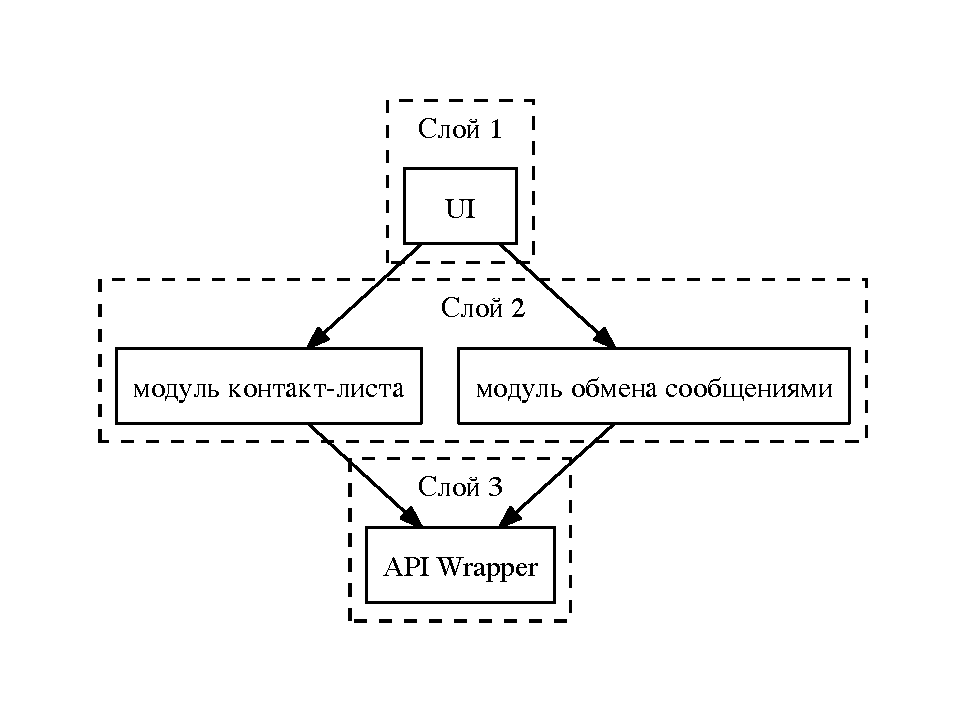
\includegraphics[width=\textwidth]{./pics/logic.pdf}
\end{frame}

\begin{frame}{Простая схема}
\begin{center}
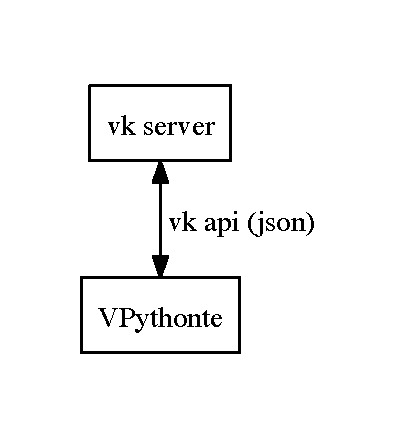
\includegraphics{./pics/simple.pdf}
\end{center}
\end{frame}

\begin{frame}{Немного про API}
\begin{itemize}
\item<1-> Для использования API требуется авторизация
\item<2-> 3 запроса в секунду от каждого уникального пользователя, запустившего приложение
\item<3-> Вечером сервер долго отвечает
\end{itemize}
\end{frame}


\begin{frame}{Пример функции запроса к API}
\lstinputlisting{./src/api_input.py}
\end{frame}


\begin{frame}{Пример ответа сервера}
\lstinputlisting{./src/api_output.py}
\end{frame}

\begin{frame}{Схема чуть сложнее}
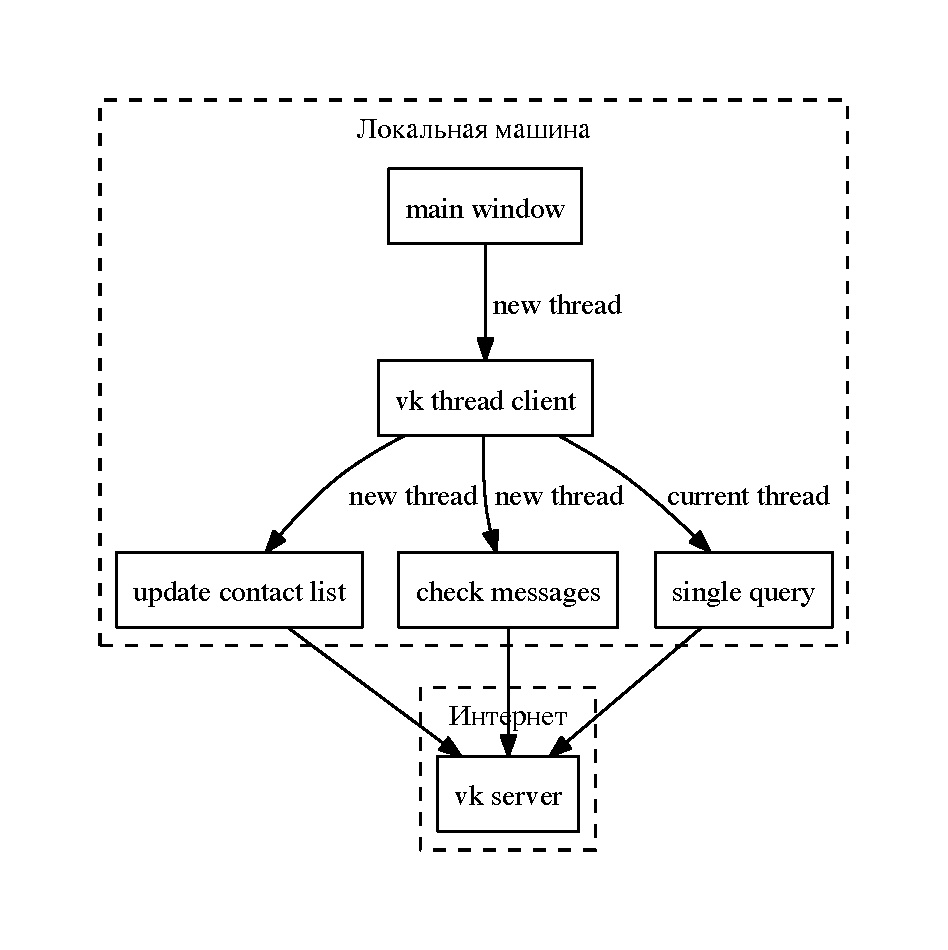
\includegraphics[width=\textwidth, height=\textheight]{./pics/complex.pdf}
\end{frame}

\begin{frame}{Сложности: работа с API}
Для более удобной работы с API была написана обертка над методами
\end{frame}

\begin{frame}{Сложности: работа с сетью}

\begin{block}{Проблема}
В первой версии интерфейс <<замораживался>>, пока сервер отвечал на запрос
\end{block}

\begin{block}{Решение}
Несколько тредов. Как только сервер отвечает, интерфейс обновляется по событию.
\end{block}

\end{frame}


\begin{frame}{Сложности: работа с сетью}

\begin{block}{Проблема}
Соединение отваливается по таймауту и другие <<радости>> работы с сетью.
\end{block}

\begin{block}{Решение}
Декоратор для обработки ошибок работы с сетью и переподключения.
\end{block}
\end{frame}

\begin{frame}{Пример: декоратор}
\lstinputlisting{./src/decorator_example.py}
\end{frame}


\begin{frame}{Пример: использование декоратора}
\lstinputlisting{./src/decorator_use_example.py}
\end{frame}


\begin{frame}{Сложности: хранение настроек}

\begin{block}{Проблема}
Нужно иметь доступ и обновлять настройки из нескольких классов и тредов приложения.
\end{block}

\begin{block}{Решение}
Шаблон <<регистр>>.
\end{block}
\end{frame}



\end{document}

